%%%%%%%%%%%%%%%%%%%%%%%%%%%%%%%%%%%%%%%%%%%%%%%%%%%%%%%%%%%%%%%%%%% 
%                                                                 %
%                            CHAPTER                              %
%                                                                 %
%%%%%%%%%%%%%%%%%%%%%%%%%%%%%%%%%%%%%%%%%%%%%%%%%%%%%%%%%%%%%%%%%%% 

\chapter{Literatuurstudie}

Vooraleer een oplossing  kan worden ontworpen voor een probleem is het van belang de nodige informatie te verzamelen over de huidige staat van het probleem en eventuele reeds bestaande oplossingen. In dit hoofdstuk zal er onder andere worden gekeken naar de technologieën die op dit moment in de wetenschap gebruikt worden en welke technologieën mogelijk een oplossing kunnen bieden voor het probleem. 
\par
Het lezen van dit hoofdstuk is aangeraden aangezien het enkele belangrijke begrippen en technologieën beschrijft waarnaar zal worden verwezen in dit onderzoek. Het is echter mogelijk dit hoofdstuk over te slaan als deze informatie reeds gekend is of als de theorie achter het proces minder van belang is.
\par
Omdat dit onderzoek zich deels afspeelt binnen de wereld van kristallografie, een specifieke tak van de wetenschap, zal de eerste sectie van dit hoofdstuk gewijd worden aan het overlopen van enkele begrippen die van belang zullen zijn in het verdere verloop van het onderzoek. Daar kristallografie een eerder complexe wetenschap is, zal deze tekst een vereenvoudigde beschrijving zijn. Voor een meer accurate beschrijving wordt er verwezen naar de literatuur waarop deze sectie gebaseerd is \citep*{CRYS1}. De tweede sectie zal het Crystallographic Information File of CIF-formaat beschrijven. Dit tekstformaat ligt aan de basis van het digitaliseren van kirstalstructuren en zal gebruikt worden bij het inlezen van kristaldata. In de derde sectie wordt gekeken naar welke programma’s op dit moment worden gebruikt bij het visualiseren van kristallen en hoe deze werken. De vierde sectie kijkt naar enkele reeds bestaande CIF-parsers en of deze al dan niet kunnen gebruikt worden in dit onderzoek. Sectie vijf zal zich verdiepen in de werking van Blender en de Blender API. In de zesde en laatste sectie wordt een conclusie getrokken uit de verkregen informatie.


\section{Kristallografie}

\subsection{Wat is kristallografie}
Kristallografie kan beschreven worden als de studie van materie in een kristallijne staat en houdt zich onder andere bezig met de synthese en opbouw van kristallen en hun fysische en chemische eigenschappen. Eerder in dit hoofdstuk werd kristallografie beschreven als een specifieke tak van de wetenschap, het is echter vermeldenswaardig dat dit een erg omvattende studie is. Kristallen komen namelijk voor in vrijwel elk ander wetenschappelijk domein. Tabel[2.1] toont enkele voorbeelden van kristallen en de respectievelijke tak van de wetenschap waar deze onder vallen.
\par
In dit onderdeel zullen verder enkel de kristallografische begrippen worden beschreven die binnen de omvang van deze thesis vallen.  
\par
\begin{table}
\caption{Kristallen in wetenschappelijke takken}
\begin{tabular}{@{}ccccl@{}}
\toprule
\multicolumn{1}{c}{\textbf{Biologie}} & \multicolumn{1}{c}{\textbf{Chemie}} & \multicolumn{1}{c}{\textbf{Farmacologie}} & \multicolumn{1}{c}{\textbf{Geologie}} &  \\ \midrule
proteïnes                              & rubber                               & alle vaste medicijnen                      & alle mineralen                         &  \\
polysacharides                         & benzeen                              & vitamines                                  & metalen                                &  \\
beenderen                              & naftaleen                            &                                            &                                        &  \\ \bottomrule
\end{tabular}
\end{table}

\subsection{De eenheidscel}
Alle kristallen zijn gedefinieerd als een periodische schikking van atomen, ionen of moleculen. Het opbouwen van een kristal wordt gedaan aan de hand van roosterpunten. Een aantal roosterpunten op een lijn met een gelijke onderlinge afstand wordt een roosterlijn genoemd, een verzameling van evenwijdige roosterlijnen met eenzelfde onderlinge afstand is een roostervlak. Ten slotte kan dit worden herhaald in een derde dimensie en wordt er een roosterruimte gevormd, welke in zwart getekend staat op Figuur[2.1]. Een roosterruimte kan in essentie zo groot zijn als het beschreven kristal. Zoals eerder ook gezegd is een kristal periodisch, dit wil zeggen dat er enkel moet gekeken worden naar het kleinste unieke volume van een kristal. Dit uniek volume valt volledig binnen de roosterruimte beschreven door de eerste acht roosterpunten. Het volledige kristal kan worden opgebouwd door de translatie van deze eenheidscel in 3 richtingen in de ruimte. Een kristal bestaat gewoonlijk uit een groot aantal van deze eenheidscellen.
\par
Geometrisch gezien bevat een eenheidscel 3 paar evenwijdige parallellogrammen als omhullende vlakken en kan het beschreven worden aan de hand van 6 variabelen, welke de roosterparameters worden genoemd.  De parameters a, b en c bepalen de lengte tussen de roosterpunten volgens de drie assen van de roosterruimte . De drie resterende  variabelen worden gebruikt om de hoeken tussen deze assen te beschrijven en worden \textalpha, \textbeta{} en \textgamma{} genoemd. Deze variabelen staan ook aangeduid op Figuur[2.1] met de eenheidscel in rood. 

\begin{figure}
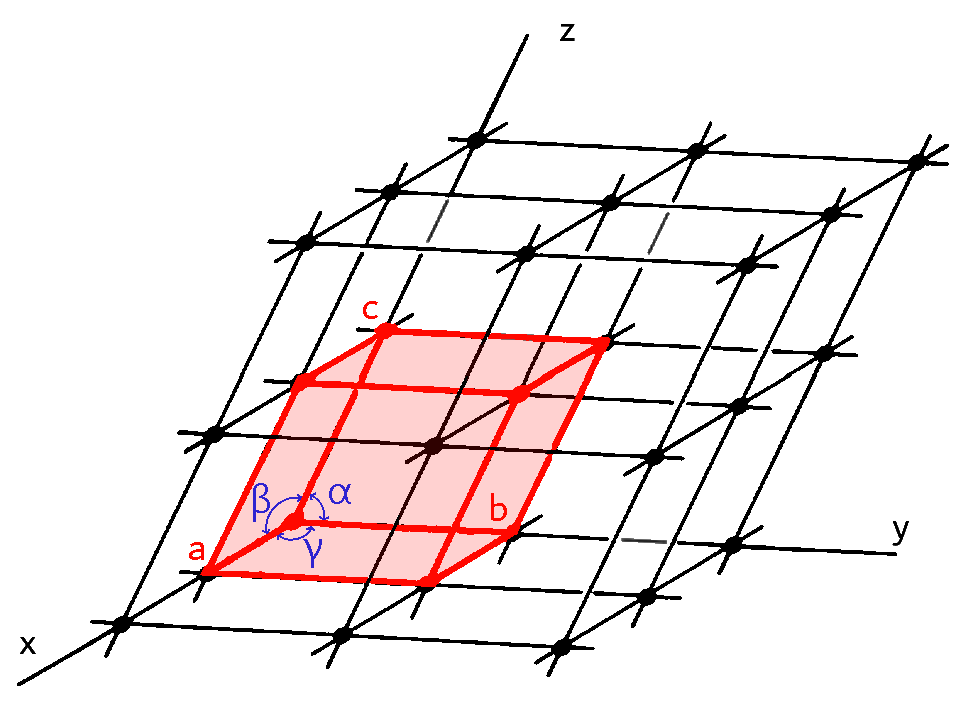
\includegraphics[scale=0.3]{roosterruimte.png}
\caption{Voorstelling van een eenheidscel in de roosterruimte \citep*{CRYS1}}
\end{figure}

\subsection{Classificatie van kristalroosters}
De vorm van de eenheidscel van een kristal is niet willekeurig, omdat dit volume de ruimte volledig moet kunnen vullen. Mogelijke types van eenheidscellen kunnen worden herleid op basis van de vorm van het vlak dat deze beschrijft, zie kolom a van Figuur[2.2]. De driedimensionale eenheidscel kan dan worden verkregen door de extrusie van dit vlak in de derde dimensie, zie kolom c van Figuur[2.2]. Zo bestaan er exact zes coördinaatsystemen, gebaseerd op de restricties van de roosterparameters. Deze vormen de basis voor de classificatie in kristalfamilies en krijgen de naam: kubisch, tetragonaal, orthorhombisch, monoclinisch, triclinisch, en hexagonaal. Deze worden weergegeven in kolom b van Figuur[2.2]. 

\par 
Vertrekkende van de mogelijke coördinaatsystemen en rekening houdend met mogelijke symmetrieën ontstaan er zeven kristalsystemen, zie kolom a van Figuur[2.3]. Hierbij wordt het hexagonale coördinatenstelsel verder opgesplitst in het trigonale en hexagonale kristalsysteem, afhankelijk van de aanwezigheid van een drie- of zesvoudige symmetrie. De zeven resulterende primitieve eenheidscellen beschrijven  voor de zeven kristalsystemen alle mogelijke eenheidstranslaties in de richtingen van x, y en z. Dit wil zeggen dat een atoom of molecule op een positie (x,y,z) ook altijd aanwezig zal zijn in de richtingen van x, y en z als de afstand identiek is aan een veelvoud van de eenheidstranslaties in deze richtingen.

\begin{figure}[H]
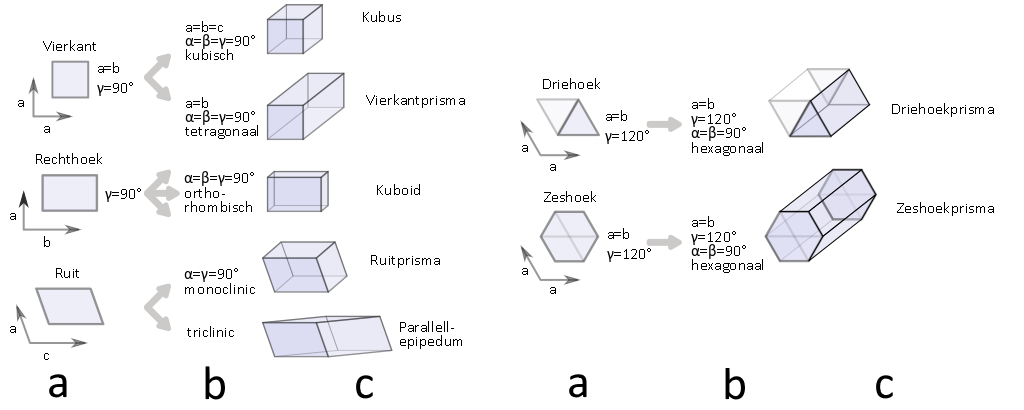
\includegraphics[scale=0.6]{families.png}
\caption{De 6 kristalfamilies}
\end{figure}

\par   
De Franse natuurkundige Bravais \citep*{BRAV} geeft een extra indeling op basis van mogelijke translaties binnen de eenheidscel, welke in overeenkomst met de symmetrievoorwaarden van de kristalsystemen zijn. Dit leidt tot de 14 Bravaisroosters, ook wel gecentreerde roosters genoemd welke worden beschreven met een letter. 
De eerste wordt de primitieve genoemd en krijgt de letter P toegekend. Bij deze bestaan alleen de eenheidstranslaties. Het rooster bevat alleen roosterpunten op de 8 hoeken van de cel.
\\
Het tweede gecentreerde rooster noemt men grondvlakgecentreerd. Deze heeft naast de eenheidstranslaties ook een centrering in een vlak. Elk deeltje kan ook teruggevonden worden over een translatie van een halve lengte langs twee assen. Er kan sprake zijn van A, B of C centrering als de verschuiving langs de diagonaal van respectievelijk het bc-, ac- of ab- vlak aanwezig is. Ondanks dit verschil worden ze niet als aparte gecentreerde roosters beschouwd.   
\\
Wanneer er extra roosterpunten liggen in elk van voorgaande vlakken spreekt men van een vlakgecentreerd of F-rooster. 
\\
Ten slotte kan er zich, naast de roosterpunten op de hoeken, ook een in het centrum van het rooster bevinden, in dit geval wordt er van een ruimtegecentreerd of I-rooster gesproken. 
\\
In het geval van het trigonale kristalsysteem bestaat er een speciale vorm van centrering in overeenkomst met de drievoudige symmetrie, welke R-centrering genoemd wordt. Kolom b van Figuur[2.3] geeft de 14 resulterende Bravaisroosters weer, dit zijn alle mogelijke vormen dat een kristal kan aannemen.
 
\begin{figure}[H]
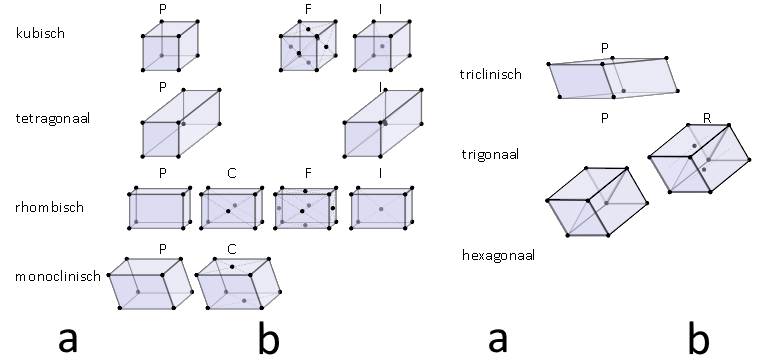
\includegraphics[scale=0.6]{Bravais.png}
\caption{De 14 Bravaisroosters en hun kristalsystemen}
\end{figure}

\subsection{Ruimte- en puntgroepen}
Dit concept is vrij complex en minder van belang voor dit onderzoek. Omdat gerelateerde termen in het verloop van deze tekst aan bod komen is het toch best deze beknopt toe te lichten. In deze literatuurstudie zal de exacte theorie hierachter niet in detail beschreven worden, maar enkel wat er van belang is voor het begrijpen van deze thesis.

\par
Puntgroepen wijzen op de innerlijke symmetrie van een roosterpunt. Een puntgroep kan gezien worden als een verzameling van symmetrieoperaties. Een symmetrieoperatie wordt als een manipulatie van een object beschouwd welke het object in zijn oorspronkelijke vorm transformeert. Naast de identiteit van een object met zichzelf zijn er vier verschillende soorten van symmetrieoperaties: spiegeling in een vlak , rotatie rond een as, inversie en de combinatie van een spiegeling en een inversie, wat een draai-inversie wordt genoemd. In totaal bestaan er 32 kristallografische puntgroepen, welke in overeenkomst zijn met de symmetrievoorwaarden van de 7 reeds besproken kristalsystemen. 

\par
Ruimtegroepen kijken niet enkel naar innerlijke symmetrie maar ook naar de symmetrie van de kristalstructuren en worden verkregen door de puntgroepen toe te passen op de 14 reeds gekende Bravaisroosters. Dit leidt tot in theorie 448 combinaties, maar door de gelijkenis tussen sommige is dit nummer terug te brengen naar een totaal van 230 ruimtegroepen. Dit heeft als gevolg dat er 230 verschillende manieren bestaan om deeltjes te ordenen in een eenheidscel. Als gevolg kan elk kristal altijd in een van deze ruimtegroepen beschreven worden. 

\subsection{Beschrijving van een kristal}
Met voorgaande informatie in het achterhoofd is het mogelijk een kristalstructuur te beschrijven. De enige informatie die hiervoor nodig is, is de ruimtegroep, het gebruikte coördinaatsysteem en de mogelijke centrering die alle symmetrieoperaties definieert. Vervolgens worden de roosterparameters van de eenheidscel gegeven en de lijst van elementen waarop deze symmetrieoperaties geldig zijn. Ten slotte kan er ook een lijst worden gegeven van alle atomen die niet door het uitoefenen van de gegeven symmetrieoperaties geplaatst kunnen worden. Deze symmetrieonafhankelijke atomen in hun elementaire cel worden een asymmetrische eenheid genoemd. Met voorgaande gegevens kan elk mogelijk kristal afgebeeld en beschreven worden. 

\subsection{Het fractionele coördinatensysteem}
De positie van atomen binnen het eenheidskristal wordt meestal beschreven aan de hand van zijn x-, y- en z-waarden. Deze waarden stellen steeds hun relatieve positie voor ten opzichte van de respectievelijk a- b- en c-waarden van de roosterparameters, vandaar de naam fractioneel, en liggen steeds tussen nul en een. Het gebruik van het fractionele systeem heeft als groot voordeel dat het erg eenvoudig te interpreteren is, zo hoeft er geen rekening gehouden te worden met de hoeken tussen de assen van het eenheidskristal. Een element met waarden ($\frac{1}{2}$,$\frac{1}{2}$,$\frac{1}{2}$) ligt dus bijvoorbeeld in het midden van het kristal, terwijl een met waarden (1,1,1) het hoekpunt van het rooster inneemt dat zich diagonaal tegenover de oorsprong van het rooster bevindt, Figuur[2.4].
\par
\begin{figure}[H]
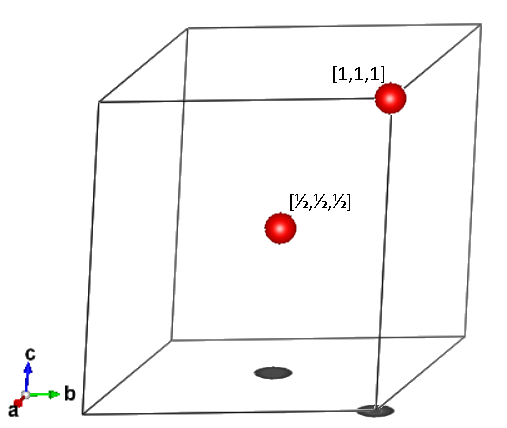
\includegraphics[scale=0.5]{FractionalExample.png}
\caption{Twee elementen in een rooster met hun fractionale coördinaten}
\end{figure}
\par
Het fractionele coördinatensysteem brengt natuurlijk ook enkele nadelen met zich mee. Om een kristal, en zijn elementen, weer te geven als een driedimensionaal figuur is er nood aan coördinaten volgens het orthogonale systeem, hiervoor kunnen de fractionele coördinaten dus niet gebruikt worden. Er zouden enkel waarden tussen nul en één kunnen verkregen worden wat telkens zou leiden tot een kubusvormig kristal. Deze foute dimensionering kan worden vermeden door deze te vermenigvuldigen met de lengte van hun respectievelijke as van het kristalrooster. Dit laatste biedt slechts deels een oplossing voor de omzetting van het fractioneel naar het orthogonaal coördinatensysteem en is enkel van toepassing voor kubische, tetragonale en orthorhombische kristalroosters aangezien deze uitsluitend bestaan uit rechte hoeken. Om een algemene formule op te stellen die gebruikt kan worden bij deze conversie moet er ook rekening gehouden worden met de hoeken tussen de assen van het kristalrooster. De algemene formule wordt voorgesteld als een matrix en ziet er voor een kristal met roosterparameters a, b, c, \textalpha, \textbeta{} en \textgamma{} uit als volgt. 
\par
\[
\begin{bmatrix}
    a & b \cdot cos(\gamma) & c \cdot cos(\beta) \\
    0 & b \cdot sin(\gamma) & c \cdot \dfrac{cos(\alpha)-cos(\beta) \cdot cos(\gamma)}{sin(\gamma)}  \\
    0 & 0 & \dfrac{\Omega}{a \cdot b \cdot sin(\gamma)}\\
\end{bmatrix}
\]
\par
\[
Met\; \Omega{}\; het\; volume\; van\; de\; eenheidscel.
\]
\par
\[
\Omega{} = a\cdot b \cdot c \cdot \sqrt{1-cos^2(\alpha) - cos^2(\beta) - cos^2(\gamma) + 2 \cdot cos(\alpha) * cos(\beta) \cdot cos(\gamma)}
\]
\par 
De orthogonale coördinaten van een element kunnen dan als volgt worden berekend:
\par
\[
\begin{bmatrix}
    x_{orth} \\
    y_{orth} \\
    z_{orth} \\
\end{bmatrix}
=
\begin{bmatrix}
    a & b \cdot cos(\gamma) & c \cdot cos(\beta) \\
    0 & b \cdot sin(\gamma) & c \cdot \dfrac{cos(\alpha)-cos(\beta) \cdot cos(\gamma)}{sin(\gamma)}  \\
    0 & 0 & \dfrac{\Omega}{a \cdot b \cdot sin(\gamma)}\\
\end{bmatrix}
\bullet
\begin{bmatrix}
    x_{frac} \\
    y_{frac} \\
    z_{frac} \\
\end{bmatrix}
\]
\par
Deze conversiematrix kan gebruikt worden voor elk element dat behoort tot dit kristalrooster en elk ander kristal met dezelfde roosterparameters. 
\par


\section{Het Crystallographic Information File (CIF) formaat}

\subsection{Het STAR formaat}
Om een beter idee te krijgen van de syntax van het CIF-formaat worden eerst de onderliggende concepten beschreven van het Self-Defining Text Archive and Retrieval (STAR) bestandsformaat,  waarop het CIF-formaat gebaseerd is. 
\par
Het STAR-formaat was de eerste stap naar de digitalisering van verschillende soorten data. \citep*{CIF2} Dit formaat bestaat uit ASCII tekst, wat makkelijke aanpassing en leesbaarheid toelaat door zowel mensen als computers. De opbouw van dit formaat ziet er uit als volgt: een file kan bestaan uit een of meerdere datablokken, welke nogmaals onderverdeeld zijn in een sequentie van data-elementen. De identiteit van een data- element wordt bepaald door een unieke naam die ervoor wordt geplaatst in het bestand. Het kleine aantal regels in een STAR-bestand maakt dit een eenvoudig en veelzijdig formaat. Zo zijn er geen restricties op de volgorde waarin de data moet worden genoteerd en moet er geen kennis zijn van het datatype van een element. Het gebruik van een lus maakt het mogelijk de toekenning van data- elementen te herhalen.

\subsection{De CIF-notatie}   
Het CIF-formaat bouwt verder op de syntax van het reeds besproken STAR-formaat met een aantal extra voorwaarden. Enkel de datanamen die beschreven worden in de CIF-dictionary [Bijlage A] worden toegelaten, dit woordenboek bevat dan ook alle parameternamen die nodig zijn om een kristal te beschrijven. De datanamen in het CIF-woordenboek zijn opgesteld door de Internationale Unie van Kristallografie (IUCr) en zijn dus algemeen aanvaard. Een lijn in het CIF-formaat mag niet langer zijn dan 80 karakters en een datanaam niet langer dan 32. Doordat in de CIF-dictionary datanamen worden opgedeeld op basis van het item dat ze beschrijven, is dit echter geen probleem. Net zoals bij de STAR-notatie is er geen verplichting tot het toekennen van datatypes, dit wordt bij het CIF-formaat echter wel aangeraden om de datawerking vlotter te laten verlopen. Zo worden data-elementen gezien als nummers wanneer ze beginnen met een cijfer. Een nummer kan een geheel getal , een kommagetal of als wetenschappelijke notatie worden gegeven. In het CIF-woordenboek worden ook de standaardeenheden van de data-elementen bijgehouden, de afmetingen van een eenheidscel worden verondersteld in Ångström te zijn. De Ångström is een eenheid die vaak gebruikt wordt in kristallografie en heeft de waarde van 0,1 nanometer. Data wordt beschouwd als tekst wanneer deze langer is dan één lijn. In het geval dat een data-element noch een nummer noch tekst is, wordt het beschouwd als een karakter. 

\subsection{Voorbeeld van een CIF-bestand}

In dit onderdeel wordt aan de hand van listings uit een CIF-bestand de betekenis van de vaak voorkomende termen uitgelegd. Deze listings zijn slechts delen van het CIF-bestand van een bestaand kristal [Bijlage B] en dienen enkel als voorbeeld.


\begin{lstlisting}
data_CHA
\end{lstlisting}
De naam van het datablok.
\begin{lstlisting}
#**************************************************************************
# CIF taken from the IZA-SC Database of Zeolite Structures
# Ch. Baerlocher and L.B. McCusker
#**************************************************************************
\end{lstlisting}
Alles achter een hashtag is commentaar en is enkel zichtbaar voor de lezer. 
\begin{lstlisting}
_cell_length_a                  13.6750(0)
_cell_length_b                  13.6750(0)
_cell_length_c                  14.7670(0)
_cell_angle_alpha               90.0000(0)
_cell_angle_beta                90.0000(0)
_cell_angle_gamma              120.0000(0)
\end{lstlisting}
De roosterparameters, de lengtes van de ribbes in Ångström en de hoeken tussen de assen in graden, een getal tussen haakjes achteraan wijst op de geschatte standaardafwijking van het getal. 
\begin{lstlisting}
_symmetry_space_group_name_H-M     'R -3 m'
_symmetry_Int_Tables_number         166
_symmetry_cell_setting             trigonal
\end{lstlisting}
De notatie van de ruimtegroep, het nummer van de ruimtegroep en het kristalstelsel van de eenheidscel.
\begin{lstlisting}
loop_
_symmetry_equiv_pos_as_xyz
'+x,+y,+z'
'2/3+x,1/3+y,1/3+z'
'1/3+x,2/3+y,2/3+z'
\end{lstlisting}
Deze lus geeft de posities waarop de atoomgroep worden geplaatst, deze lijst is vaak erg lang.
\begin{lstlisting}
loop_
_atom_site_label
_atom_site_type_symbol
_atom_site_fract_x
_atom_site_fract_y
_atom_site_fract_z
    O1    O     0.9020    0.0980    0.1227
    O2    O     0.9767    0.3101    0.1667
    T1    Si    0.9997    0.2264    0.1051
\end{lstlisting}
Deze lus beschrijft de groep van atomen en waar deze zich bevinden in het kristal. De eerste twee data-elementen bepalen respectievelijk het zelfgekozen symbool voor het element en de wetenschappelijke afkorting van het chemisch element. De drie laatste waarden geven de relatieve positie van deze atomen binnen de eenheidscel ten opzichte van de lengte van de ribben.

\subsection{Kristallografische databanken}
Aangezien het CIF-formaat gezien kan worden als een standaardformaat voor het beschrijven van kristallen bestaan er reeds CIF-bestanden voor vrijwel alle bestaande kristalstructuren. De verzameling van deze bestanden, alsook andere formaten, worden kristallografische databanken genoemd en staan online ter beschikking op verschillende websites. De lijst met kristalstructuren blijft groeien en wordt bijgewerkt door verschillende organisaties en universiteiten. Een voorbeeld hiervan is de Crystallography Open Database (COD) waar de kirstalstructuren van onder andere organische, anorganische en metaalorganische samenstellingen kunnen teruggevonden worden. Het voorbeeldbestand in vorige sectie is een deel van de beschrijving van de kristalstructuur van het zeoliettype Chabaziet, dit CIF-bestand kan teruggevonden worden in de zeolietstructuurdatabank op de website van de International Zeolite Association (IZA) welke zich uitsluitend bezighoudt met het onderzoeken en beschrijven van de verschillende types van het mineraal zeoliet.

\section{Kristalvisualisatiesoftware}

\subsection{Visualization for Electronic and Structural Analysis (VESTA) 3}
Als een van de meest frequent gebruikte 3D visualisatieprogramma’s biedt VESTA 3 een grotere verscheidenheid aan features en voordelen dan zijn voorgangers en andere, gelijkaardige programma’s doen. VESTA beschrijft zichzelf als een gratis te gebruiken 3D visualisatiesysteem voor structurele modellen, volumetrische data en kristalmorfologieën. \citep*{VESTA1} De software wordt ondersteund op Windows, Mac en Linux. Geschreven in de programmeertaal C met het gebruik van de OpenGL technologie en een modern C++ GUI framework biedt VESTA een gebruikersvriendelijke interface met de mogelijkheid tot het roteren, transleren en schalen van het getekende object alsook het hierop plaatsen van fysieke gegevens zoals elektronendichtheden, nucleaire dichtheden, golffuncties en elektrostatische potentialen. Hiernaast bestaan er verschillende manieren om het object weer te geven. De omvang van deze objecten is in theorie oneindig en wordt slechts beperkt door de hardware van de computer, hoe groter het grafische rekenvermogen van deze hoe vlotter het zal functioneren. De grafische interface van VESTA wordt weergegeven op Figuur[2.5]. VESTA is in staat verschillende bestandsformaten om te zetten naar een driedimensionale voorstelling, zoals het CIF-formaat. VESTA laat toe nieuwe modellen aan te maken of bestaande modellen aan te passen. Gecreëerde objecten kunnen ten slotte geëxporteerd worden in de meest voorkomende 3D formaten zodat ze in andere 3D software, zoals Blender, kunnen worden bekeken.
\\
\begin{figure}[H]
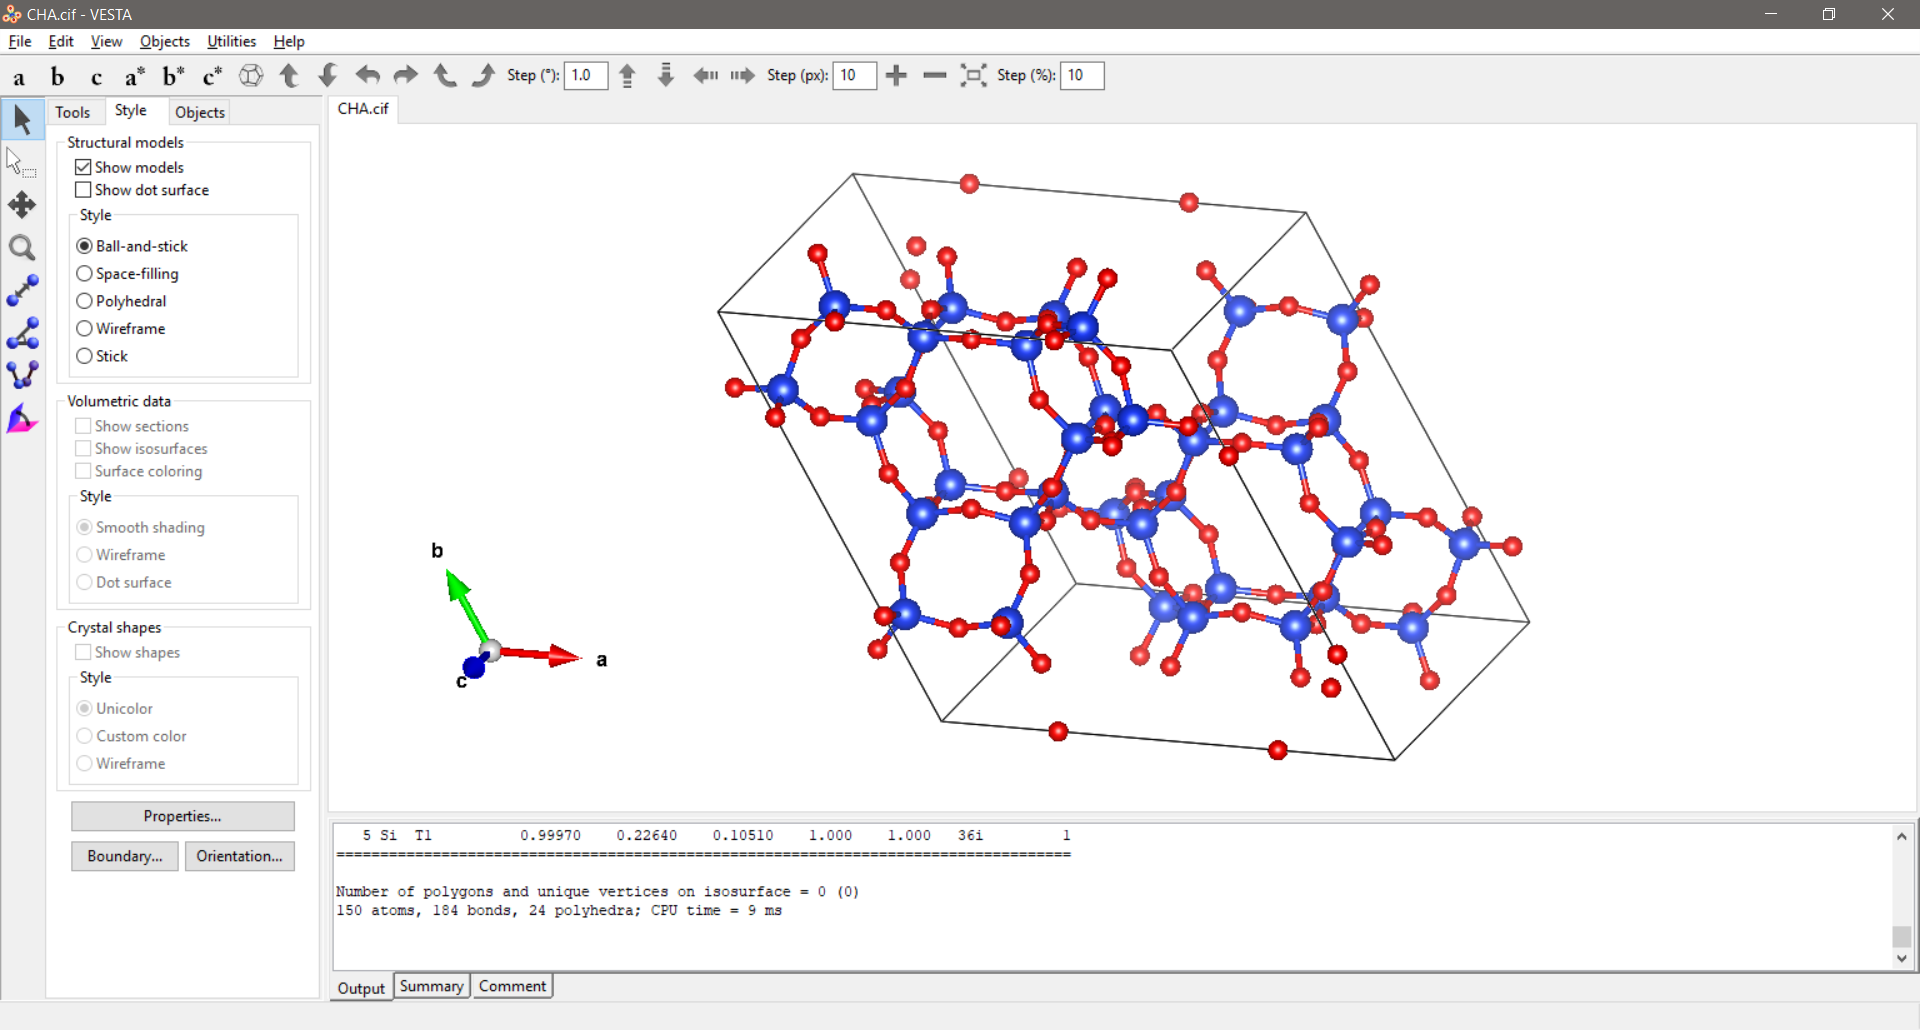
\includegraphics[scale=0.2]{VESTA-UI.png}
\caption{De user interface van VESTA3}
\end{figure}

\par
 Omdat de broncode van VESTA niet openbaar beschikbaar is, is het vrijwel onmogelijk eigen features toe te voegen, en hangt de gebruiker vast aan de tools die deze software ter beschikking stelt. Deze beperking aan vrijheid heeft ertoe geleid dat wetenschappers op zoek gaan naar andere software die dit wel aanbiedt.

\subsection{Andere 3D visualisatiesoftware}
Naast VESTA bestaat er nog een groot aanbod aan andere software die in staat zijn kristallen driedimensionaal te visualiseren. Het Crystalmaker softwarepakket biedt het programma Crystalviewer, Figuur[2.6], gratis aan voor persoonlijk gebruik. Het strak design en de gebruiksvriendelijke user interface geven de software een luxueus gevoel. Voor het gebruik van het volledig potentieel van dit programma en om toegang te krijgen tot de documentatie wordt de gebruiker ertoe gedwongen het eerder dure, volledige softwarepakket aan te kopen. Hiernaast biedt de gratis versie niet de mogelijkheid andere formaten in te lezen dan het .crystal – formaat, wat niet gezien wordt als standaardformaat en niet bestaat in de kristallografische databanken. 

\begin{figure}[h]
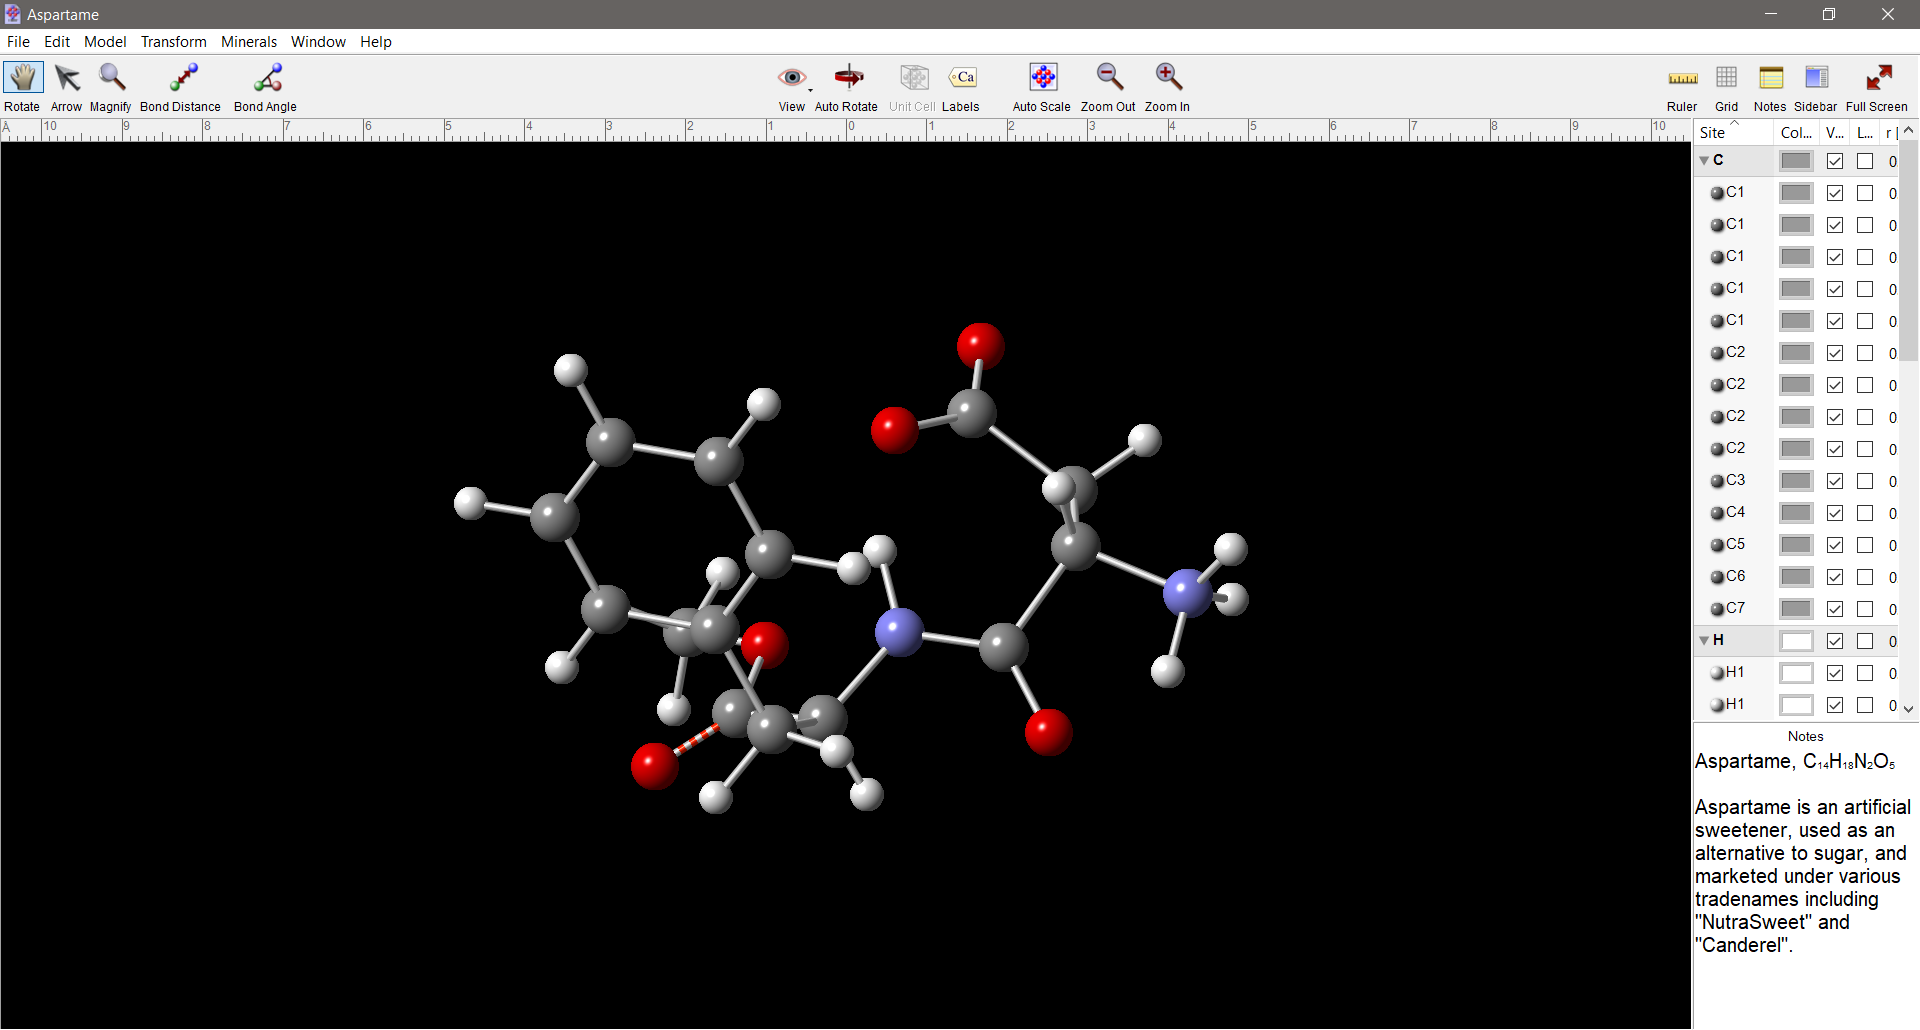
\includegraphics[scale=0.2]{Crystalviewer9-UI.png}
\caption{De user interface van Crystalviewer9}
\end{figure}

\par
Een andere bekende tegenhanger van VESTA is Olex\textsuperscript{2}, zie Figuur[2.7]. Olex\textsuperscript{2} biedt, net zoals VESTA, een groot aantal features aan, welke duidelijk beschreven worden in een overzichtelijke documentatie. Het softwarepakket is volledig gratis en ter beschikking van iedereen. Olex\textsuperscript{2} is volledig geschreven in Python en maakt gebruik van enkele bibliotheken die de gebruiker de mogelijkheid biedt verschillende kristalbeschrijvingsformaten, waaronder CIF, in te lezen en te visualiseren. Ondanks de features en documentatie is het gebruiken van Olex\textsuperscript{2} minder eenvoudig dan de eerder geziene programma’s. Bij het testen van dit programma trad er ook een probleem op bij het visualiseren van een CIF-bestand, wat deze software voor deze toepassing vrijwel onbruikbaar maakt.

\begin{figure}[h]
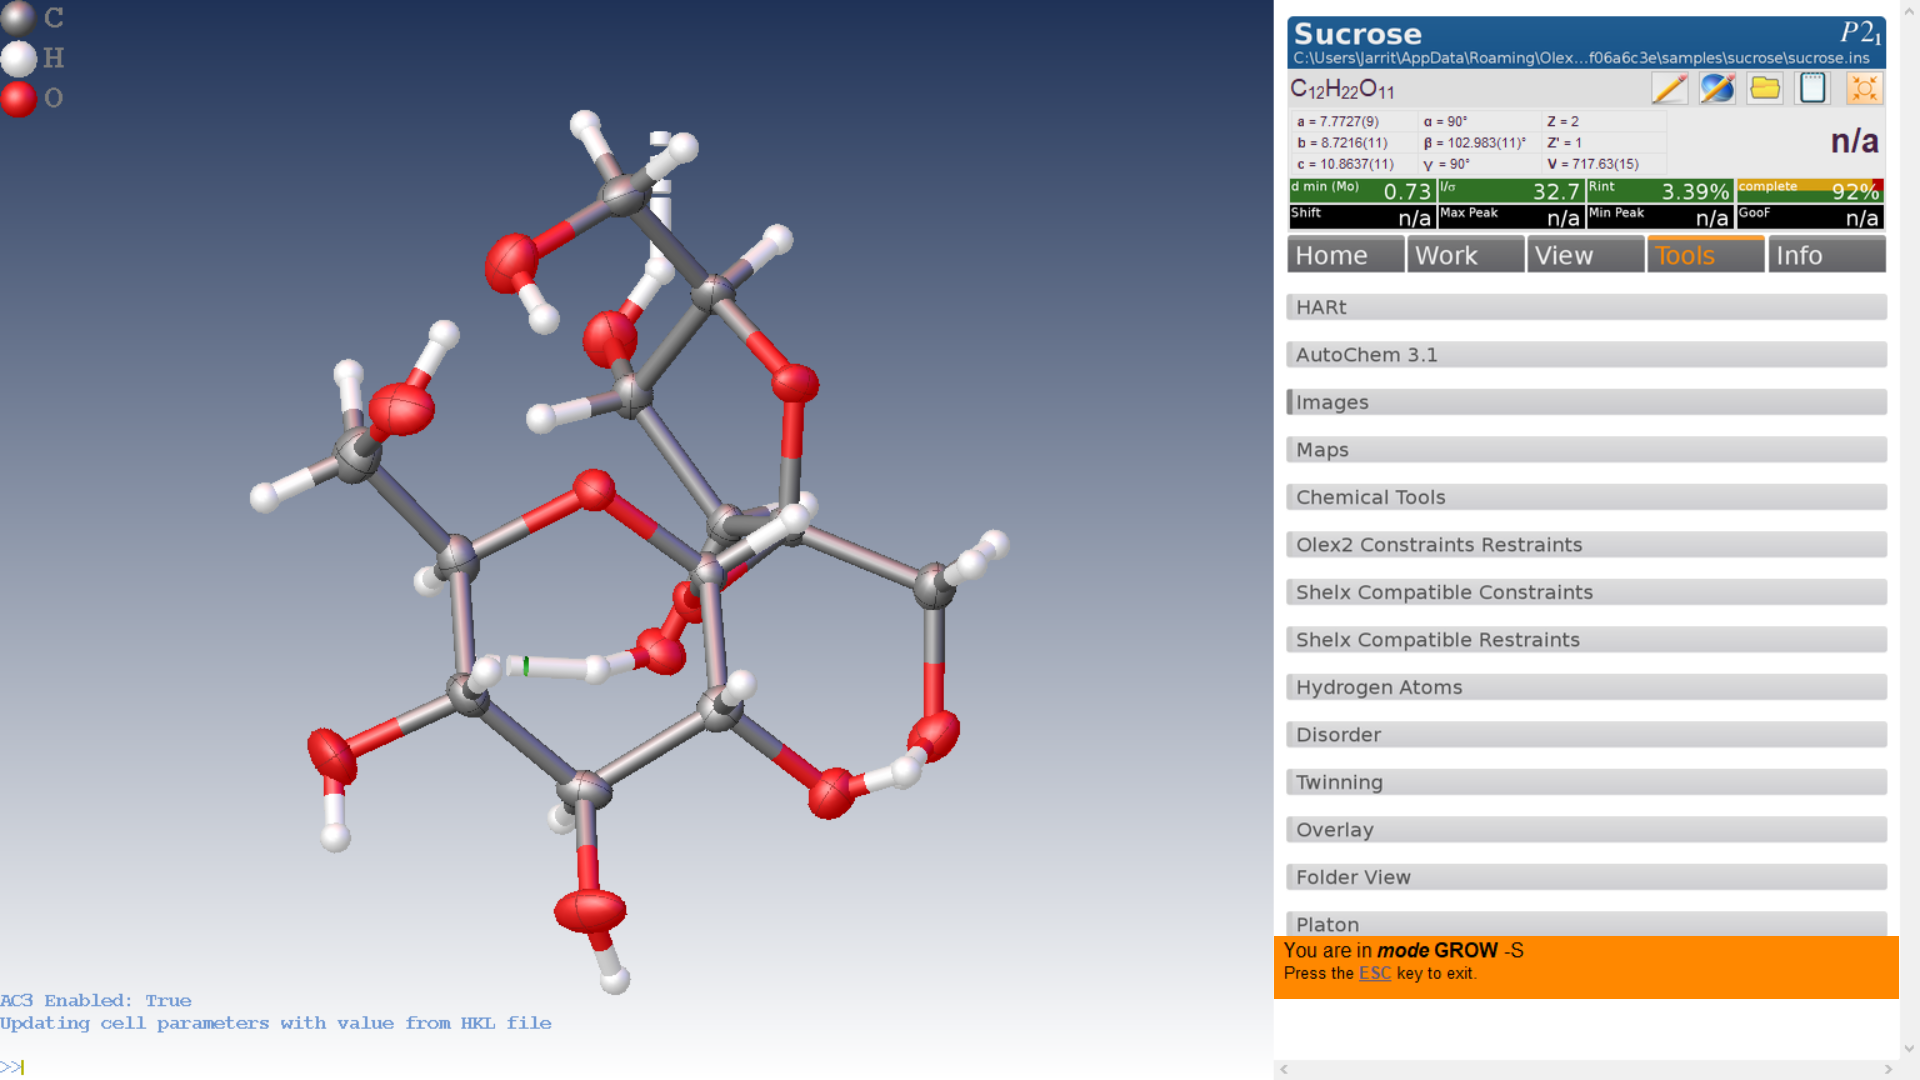
\includegraphics[scale=0.2]{Olex2-UI.png}
\caption{De user interface van Olex\textsuperscript{2}}
\end{figure}

\section{CIF-Parsers}
\subsection{Wat is een parser}
Een parser wordt gezien als een computerprogramma of script dat in staat is een input om te zetten naar een datastructuur met als voorwaarden dat deze input volgens een bepaalde structuur, denk XML, is ingegeven. De parser gaat in de ingevoerde gegevens op zoek naar herkenbare elementen en slaat deze op volgens een eerder genoemde datastructuur, bijvoorbeeld een boomstructuur of een dictionary. Sommige parsers worden gebruikt om ingegeven data te visualiseren, deze data kan dan worden gevisualiseerd in de vorm van een boomstructuur of een grafiek. Een ander soort van parsers heeft als nut de gegevens van het bestand om te zetten in een dictionary, waardoor deze in een ander programma eenvoudig kunnen worden opgevraagd. In dit onderzoek is er nood aan dit tweede type van parser, zodat de gegevens in een CIF-bestand kunnen worden omgezet naar door de module leesbare data. 

\par
\subsection{Het schrijven van een parser}
Om een parser te schrijven voor een bepaald bestandstype of formaat is er eerst een goede kennis nodig van dit formaat. Hoewel het op eerste zicht misschien niet logisch lijkt, wordt het schrijven van een parser eenvoudiger naarmate de striktheid van het formaat stijgt. Er moet minder rekening worden gehouden met alle mogelijke variaties die in het bestand kunnen voorkomen. Zoals in sectie twee besproken werd, bestaan er in het CIF-formaat weinig regels op vlak van tekststructuur. Hierdoor vergt het schrijven van een CIF-parser veel werk. In dit onderzoek is er aanvankelijk geprobeerd een eigen parser te ontwerpen die kan gebruikt worden om CIF-bestanden om te zetten naar bruikbare data. Dit proces wordt in hoofdstuk drie in meer detail besproken. Omdat dit echter niet het doel is van dit onderzoek, is er besloten te kijken naar de mogelijkheden die reeds bestaande CIF-parsers kunnen bieden. De bekeken parsers worden verder beschreven.  

\par
\subsection{The Computational Crystallography Toolbox (cctbx)}
Dit project heeft als voornaamste doel een brug te bouwen tussen kristallografische data en het gebruik hiervan in computer gerelateerde toepassingen. Het project is volledig open source, wat wil zeggen dat het volledig toegankelijk en gratis is voor iedereen die het wil gebruiken, hiernaast zorgt dit ervoor dat dit project voortdurend wordt verbeterd en stijgt in functionaliteit. Deze toolbox ligt ook aan de basis van de visualisatiesoftware Olex\textsuperscript{2}, welke beschreven wordt in de derde sectie van dit hoofdstuk. De grote omvang van dit project en het grote aantal functionaliteiten maakt het, ondanks de duidelijke documentatie, ook meer ingewikkeld om dit te gebruiken. 

\subsection{Python CIF Read/Write (PyCIFRW)}
Naast het inlezen van CIF-bestanden kunnen deze bestanden met dit programma ook gecreëerd en aangepast worden. Ook dit programma is open source, omdat dit op een kleinere schaal gebeurt dan cctbx, zie vorige, zijn de mogelijkheden, hoewel meer beperkt, geschikter voor gebruik in dit onderzoek. Door de goede documentatie van dit project en de volledige ondersteuning van Python kan dit programma gecombineerd worden met de, in de volgende sectie besproken, Blender API. \citep*{PYCIFRW1} Voor deze thesis is de schrijffunctie minder van belang, deze zal niet worden bekeken. 

\lstset{caption = Werken met PyCIFRW in Python3}
\lstinputlisting{listings/parservb.py}

\par 
Listing[2.7] is een voorbeeld van hoe PyCIFRW kan worden gebruikt in Python om een CIF-file in te lezen. De voornaamste functies worden hier weergegeven. Een meer gedetailleerde beschrijving van de werking van PyCIFRW kan worden teruggevonden in hoofdstuk 4.

\section{Blender en de Blender API}

\subsection{Gratis software}
Blender beschrijft zichzelf als een \enquote{open-sourced, community development program}, en is het collectieve werk van softwareontwikkelaars overal ter wereld. \citep*{BLEN1} De ontwikkeling en het correct functioneren van dit programma wordt overzien door The Blender Foundation, een Nederlandse, onafhankelijke, non-profit stichting. Dit alles leidt ertoe dat de Blender software gratis verkrijgbaar is voor iedereen die het wenst te gebruiken.

\subsection{Blender in de bedrijfswereld}
Zoals in het verdere verloop van deze sectie duidelijk zal worden, heeft Blender een groot aantal verschillende toepassingen. Hierdoor wordt Blender niet enkel door amateurs gebruikt, maar ook door bedrijven in verschillende industrieën waaronder verkoop, manufacturing, game development en vele anderen. Een voorbeeld van de kracht van Blender is Tangent Animation, een animatiestudio die uitsluiten werkt met Blender. In 2018 ontwikkelde dit bedrijf de animatiefilm Next Gen welke te zien is op onder andere Netflix, Figuur[2.8].
\par

\begin{figure}[H]

\includegraphics[width=\textwidth,keepaspectratio]{next-gen-poster.png}
\caption{Poster van de film Next Gen \citep*{NEXT1}}
\end{figure}

    



\subsection{De Blender interface}
Na het opstarten van Blender wordt de gebruiker begroet met de Blender interface. Een niet ervaren gebruiker zal, naast onder de indruk, vooral in de war zijn en niet weten waar te beginnen. In Figuur[2.9] wordt het startscherm weergegeven en worden enkele onderdelen ervan beschreven. Veel van deze tools en hoe deze werken vallen niet binnen het bestek van deze tekst en worden weinig of niet uitgelegd, hiervoor wordt verwezen naar online handleidingen en de documenten waar deze tekst op gebaseerd is.\citep*{BLEN1}\citep*{API1} 

\begin{figure}[h]
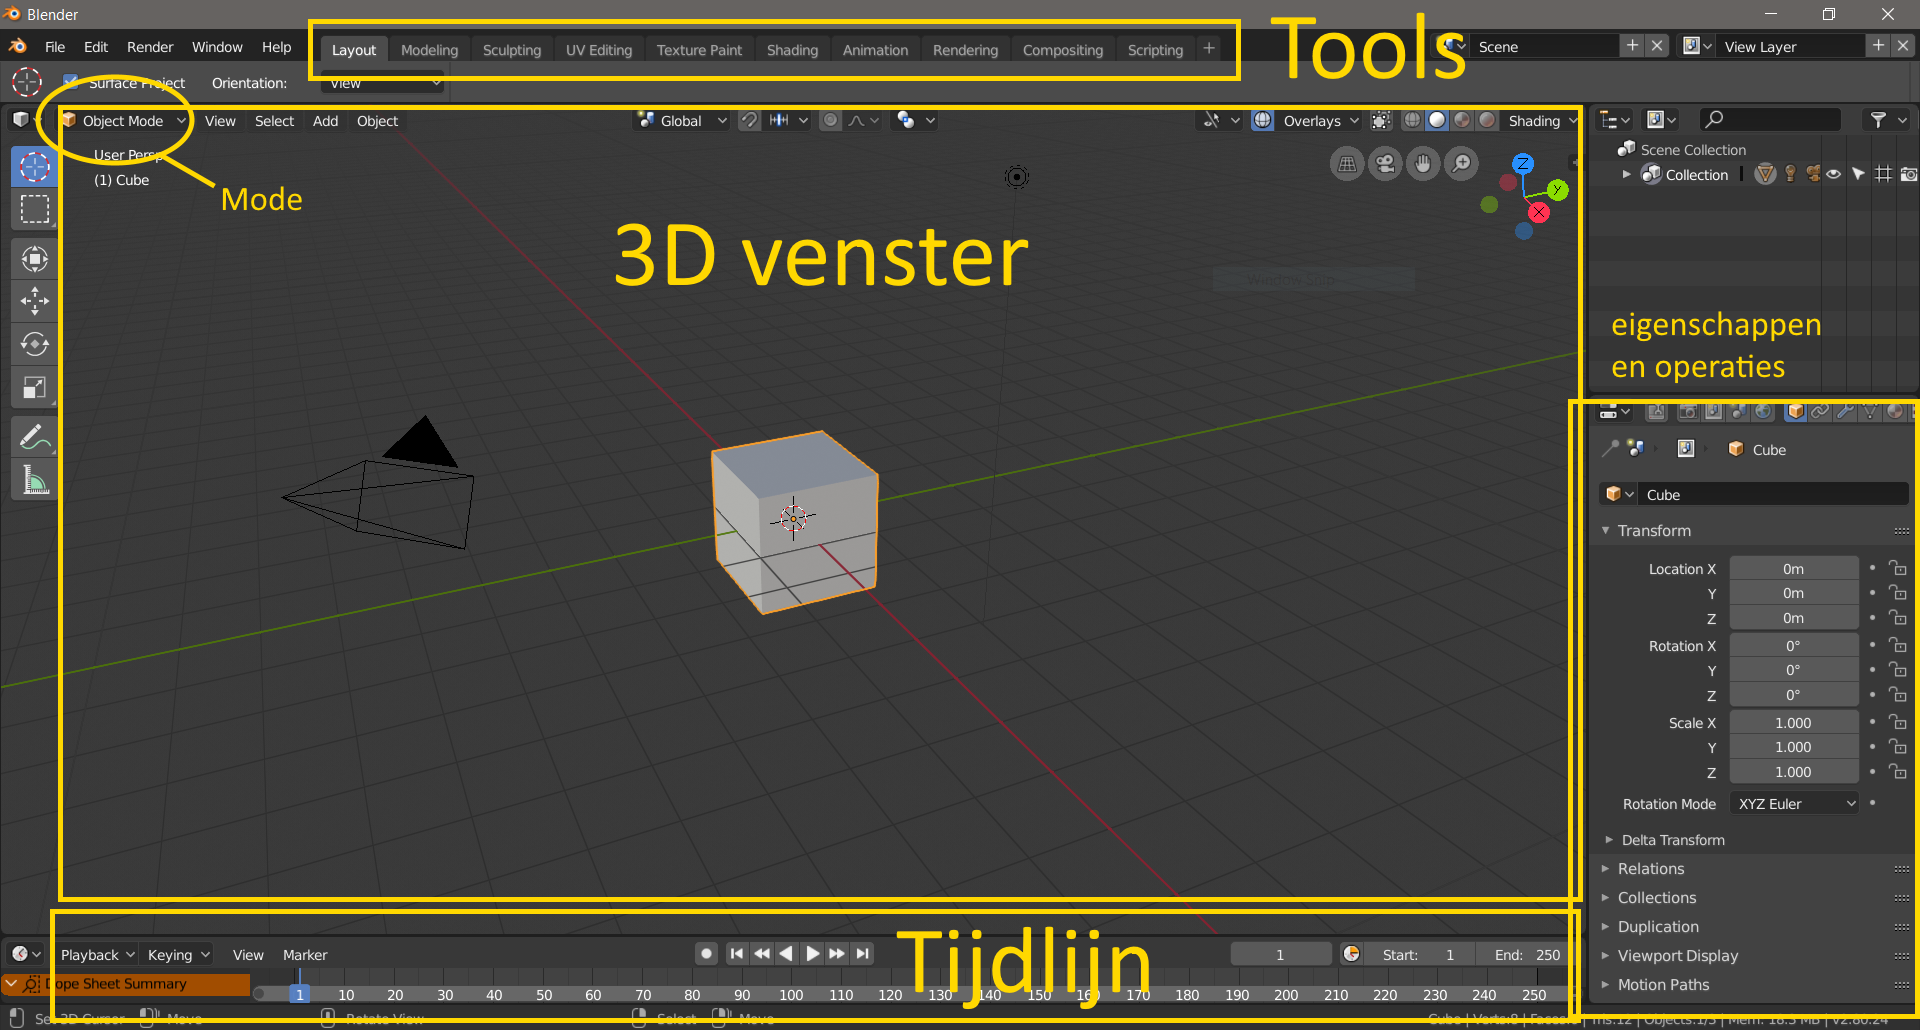
\includegraphics[scale=0.3]{Blender.png}
\caption{Het Blender startscherm}
\end{figure}

\par
In het midden van het scherm kan het 3D venster worden teruggevonden. Hier worden alle objecten weergegeven die zich op de huidige ingeschakelde layers bevinden. Het gebruik van layers laat toe objecten op een andere layer tijdelijk te verbergen om zo een duidelijk overzicht te behouden over het huidige werk. Wanneer een object wordt aangemaakt zal deze automatisch geplaatst worden op de huidige layer. De Blender interface heeft twee modes: object mode en edit mode.
\\
In object mode kan een object in zijn geheel bewerkt worden. Transleren, roteren en herschalen zijn slechts enkele van het groot aantal objectoperaties dat Blender aanbiedt. 
\\
Edit mode laat de gebruiker onder andere toe de vorm van het object aan te passen door hoekpunten aan te duiden en te verplaatsen. 
Objecten toevoegen wordt gedaan met de Add knop linksboven in het venster. 
In Blender gebruikt men de rechtermuisknop om items te selecteren en te verplaatsen. Het klikken op de linkermuisknop verplaatst de 3D cursor, dit is de plaats waar nieuwe objecten terechtkomen wanneer ze worden aangemaakt. Ten slotte kan in het 3D venster worden bewogen door het indrukken van het muiswiel.

\par
Met deze informatie kan er een object aangemaakt en verplaatst worden en kunnen er enkele basisoperaties op worden toegepast. Dit is voorlopig alles wat er over het bewerken van objecten gezegd zal worden. Dit is slechts het topje van de enorme ijsberg die Blender wordt genoemd.


\subsection{Kleuren, texturen en materialen}
Blender laat de gebruiker toe de gemaakte objecten, naast vorm, ook kleur te geven. Eerst krijgt het object een materiaal toegekend, waarna de eigenschappen van dit materiaal kunnen worden aangepast. Deze eigenschappen zijn onder andere de kleur, lichtuitstraling, weerspiegeling, schaduw en doorzichtigheid van het object. Om het object er nog realistischer te laten uitzien kan er een textuur op het object worden gezet. Deze geven het object een bepaalde oppervlaktestructuur of uiterlijk. Blender voorziet een aantal basistexturen maar de gebruiker kan zelf afbeeldingen gebruiken om het voorwerp een textuur te geven. Wanneer de objecten een kleur of textuur hebben kan de gebruiker deze renderen. Dit gaat alle lichtinteracties en schaduws berekenen, wat erg computerintensief kan zijn. In Figuur[2.10] wordt de uitkomst van het renderen van een Blender project weergegeven, door slim gebruik van texturen en materiaaleigenschappen was de ontwerper in staat een 3D tekening levensecht te laten lijken.\citep*{BLEN2}

\begin{figure}[h]
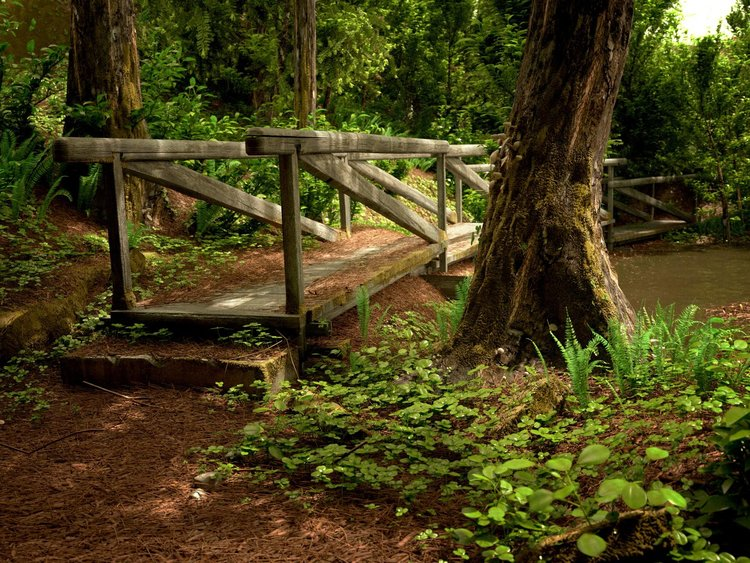
\includegraphics[scale=0.5]{blenderreal.png}
\caption{Het Blender project van de winnaar van een fotorealiteit wedstrijd, na rendering}
\end{figure}

\subsection{Andere opmerkelijke tools in Blender}
Naast het aanmaken, vervormen en inkleuren van objecten biedt Blender nog een handvol extra mogelijkheden aan. Met de Sculpting tool kan men objecten boetseren tot in de kleinste details. Dit kan leiden tot realistische beeldhouwwerken.

\par 
Onderaan de interface afgebeeld op Figuur[2.9] kan het tijdlijn-venster gezien worden. Dit venster behoort tot de animation tool van Blender, door een aantal gerenderde frames snel opeenvolgend achter elkaar te laten afspelen wordt een video verkregen. Kleine verschillen tussen deze frames geven de indruk dat het object beweegt, dit wordt een animatie genoemd. 

\par
Hoewel er betere software bestaat om dit te doen, is het in Blender, door gebruik te maken van scripts, mogelijk volledig functionele 3D videogames te ontwerpen. Zo bestaan er reeds games die volledig in Blender zijn gemaakt en te koop staan op Steam, een bekende videogames-distributeur.

\subsection{Scripten in Blender met de Blender API}
Nog een belangrijke functie die Blender aanbiedt, en in de vorige sectie niet werd vermeld, is de mogelijkheid tot het scripten in Blender zelf, in tegenstelling tot de game-engine. Omdat deze feature in zekere mate de rode draad is van deze thesis, wordt er een volledige subsectie gewijd aan dit eerder ingewikkelde onderdeel van Blender.

\par
In de tweede sectie van dit hoofdstuk werd besproken hoe operaties in Blender kunnen uitgevoerd worden met behulp van de Blender interface. Er bestaat echter een andere manier om operaties uit te voeren, namelijk via scripts. Met de juiste kennis kan er met behulp van scripts zelfs meer gedaan worden dan met enkel de interface. 
Het schrijven van scripts wordt gedaan aan de hand van Python 3, verder gerefereerd als Python. Alle standaardmodules in Python kunnen dan ook gebruikt worden, hiernaast is het mogelijk zelf modules te importen, in het geval van dit onderzoek een CIF-Parser. Aan de hand van de Python logica is het eenvoudig loops te cre\"{e} ren die automatisch een aantal objecten aanmaakt in Blender. Hieronder wordt kort de Blender API beschreven.

\par
De Blender API biedt een aantal modules aan die gebruikt kunnen worden, naast alle reeds bestaande functionaliteiten van Python. De voornaamste van deze modules is de bpy module, die alle functies bevat in verband met het aanmaken en aanpassen van objecten in Blender. De bpy module is zodanig groot dat deze nogmaals wordt opgedeeld in submodules, deze worden samen met hun taak weergegeven in tabel[2.2]. In de documentatie van de Blender API worden alle methodes van deze modules uitgelegd. In hoofdstuk vier wordt dieper ingegaan op het gebruik van de Blender API en de toepassing ervan in dit onderzoek.

\begin{table}[H]
\caption{De submodules van de Blender bpy module \citep*{API1}}
\begin{center}
\begin{tabular}{|c|l|}
\hline
\textbf{bpy.ops}                       & Bevat alle operators voor het maken en aanpassen van objecten       \\ \hline
\textbf{bpy.context}                   & Geeft de mogelijkheid specifieke data op te vragen                  \\ \hline
\textbf{bpy.data}                      & Bevat alle data van de objecten                                     \\ \hline
\textbf{bpy.app}                       & Hulpmodule bij het schrijven van add-ons en extra functionaliteiten \\ \hline
\textbf{bpy.types,bpy.utils,bpy.props} & Hulpmodules bij het schrijven van add-ons                           \\ \hline
\textbf{bpy.path}                      & Vrijwel identiek aan de os.path submodule van Python                \\ \hline
\end{tabular}
\end{center}
\end{table}


\section{Conclusie}

Kristallografie is een speciefieke tak in de wetenschap die zich bezighoudt met het onderzoeken van kristallen, hun structuur en hun eigenschappen. Een kristal wordt opgebouwd uit eenheidscellen. Het beschrijven van zo'n eenheidscel geeft alle informatie van het kristal. De vorm van een eenheidscel wordt bepaald door zes roosterparameters en een van de 14 Bravaisroosters. Deeltjes kunnen zich op 240 manieren in de eenheidscel bevinden, de ruimtegroepen genaamd.
\par
In het CIF formaat is alle informatie over een kristalstructuur terug te vinden, het is leesbaar door zowel computers als mensen. CIF bestanden worden geschreven in ASCII wat eenvoudige leesbaarheid en aanpasbaarheid toelaten. Gebaseerd op het STAR formaat heeft het CIF formaat enkele syntactische restricties waaraan moet gehouden worden. De structuur van CIF bevat datablokken, data-elementen en lussen om de data weer te geven.
\par
De bestaande 3D kristalvisualisatiesoftwarepakketten zijn vaak moeilijk in omgang, duur of bieden niet genoeg vrijheid. VESTA en Olex\textsuperscript{2} zijn gratis programma\'{}s die kristalstructuren kunnen visualiseren en geven de gebruiker een aantal handige tools om onderzoek te vereenvoudigen. Ze hebben echter hun nadelen wat leidt tot de vraag naar andere programma's.
\par
Parsers hebben als functie data te extraheren uit bestanden met een bepaalde syntax. Ze worden gebruikt om data te visualiseren of bruikbaar te maken in andere toepassingen. De complexiteit van het schrijven van een parser is omgekeerd evenredig met het aantal syntaxregels van een formaat, hierdoor is het schrijven van een CIF parser eerder moeilijk. Cctbx en PyCIFRW zijn open source modules die in staat zijn CIF bestanden te parsen.
\par
Blender is een gratis, open source project waarin driedimensionale tekeningen kunnen worden gemaakt. Met een groot aantal tools, waaronder animeren, sculpten en een eigen game-engine, geeft Blender de gebruiker veel vrijheid en mogelijke toepassingen. Door gebruik te maken van texturen en materialen kunnen er fotorealistische tekeningen gemaakt worden. Scripten in Blender laat het automatiseren van tekenen toe en wordt gedaan aan de hand van Python scripts en de modules uit de Blender API.   